% BLAKE3 tree shapes [BLAKE3, §2.1]: left subtrees are complete with a power of 2 chunks, and at
% least as big as their right siblings. Trees for 1 to 6 chunks.
% Original drawing for the Hash library.
\documentclass[tikz,border=6pt]{standalone}
\usepackage[T1]{fontenc}
\usepackage{lmodern}
% Shared style for the Hash diagrams.
% Palette: Okabe–Ito (colour-blind safe). Every diagram is drawn on an opaque white card so it
% stays legible on dark page themes.
\usetikzlibrary{arrows.meta,positioning,calc,fit,backgrounds}
\definecolor{hsblue}{HTML}{0072B2}
\definecolor{hsorange}{HTML}{E69F00}
\definecolor{hsgreen}{HTML}{009E73}
\definecolor{hsvermilion}{HTML}{D55E00}
\definecolor{hspurple}{HTML}{CC79A7}
\definecolor{hsink}{HTML}{1F2933}
\tikzset{
  >={Stealth[length=2.2mm]},
  every node/.style={font=\sffamily\small, text=hsink},
  wire/.style={draw=hsink, line width=0.6pt, ->},
  reg/.style={draw=hsink, line width=0.6pt, fill=hsblue!12, minimum width=9mm, minimum height=7mm},
  fn/.style={draw=hsink, line width=0.6pt, fill=hsorange!25, rounded corners=2pt, minimum width=10mm, minimum height=6mm},
  input/.style={draw=hsink, line width=0.6pt, fill=hsgreen!20, minimum width=9mm, minimum height=6mm},
  add/.style={circle, draw=hsink, line width=0.6pt, fill=white, inner sep=0pt, minimum size=5mm, font=\sffamily\bfseries},
  card/.style={fill=white, rounded corners=4pt},
}

\begin{document}
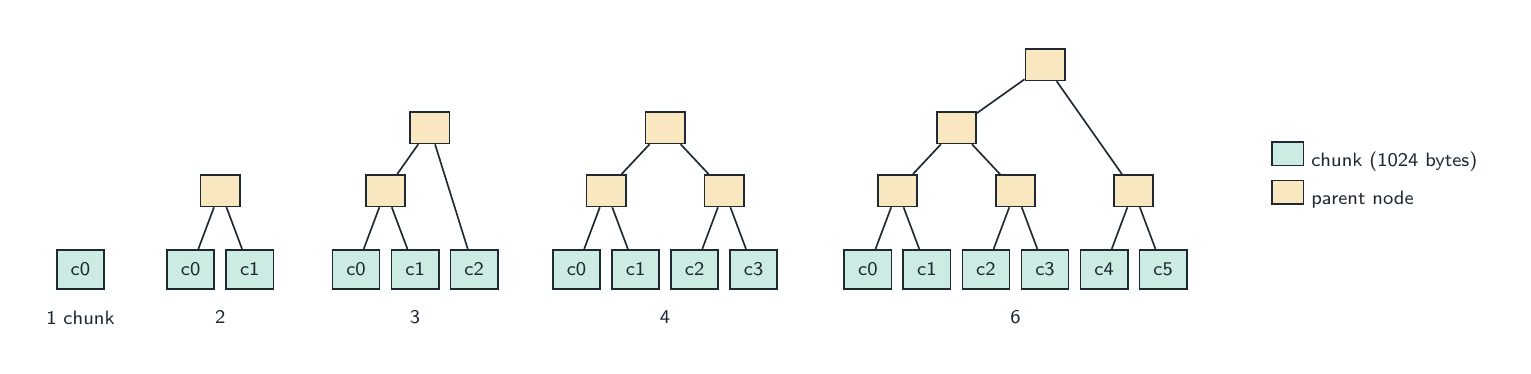
\begin{tikzpicture}[ch/.style={input, minimum width=6mm, minimum height=5mm, inner sep=1pt,
    font=\sffamily\scriptsize}, pn/.style={reg, minimum width=5mm, minimum height=4mm,
    inner sep=0pt, font=\sffamily\scriptsize, fill=hsorange!25}, e/.style={draw=hsink, line width=0.6pt}]
  \def\w{0.75}
  % Place n chunks at x offset \ox.
  \newcommand{\chunks}[3]{\foreach \i in {0,...,#3} {\node[ch] (#1\i) at (#2+\i*\w, 0) {c\i};}}
  % 1 chunk
  \chunks{A}{0}{0}
  \node[font=\sffamily\scriptsize, anchor=north] at (0, -0.4) {1 chunk};
  % 2 chunks
  \chunks{B}{1.4}{1}
  \node[pn] (p2) at (1.4+0.5*\w, 1.0) {};
  \draw[e] (p2) -- (B0); \draw[e] (p2) -- (B1);
  \node[font=\sffamily\scriptsize, anchor=north] at (1.4+0.5*\w, -0.4) {2};
  % 3 chunks: ((c0 c1) c2)
  \chunks{C}{3.5}{2}
  \node[pn] (q1) at (3.5+0.5*\w, 1.0) {};
  \node[pn] (q0) at (3.5+1.25*\w, 1.8) {};
  \draw[e] (q1) -- (C0); \draw[e] (q1) -- (C1);
  \draw[e] (q0) -- (q1); \draw[e] (q0) -- (C2);
  \node[font=\sffamily\scriptsize, anchor=north] at (3.5+\w, -0.4) {3};
  % 4 chunks
  \chunks{D}{6.3}{3}
  \node[pn] (r1) at (6.3+0.5*\w, 1.0) {};
  \node[pn] (r2) at (6.3+2.5*\w, 1.0) {};
  \node[pn] (r0) at (6.3+1.5*\w, 1.8) {};
  \draw[e] (r1) -- (D0); \draw[e] (r1) -- (D1);
  \draw[e] (r2) -- (D2); \draw[e] (r2) -- (D3);
  \draw[e] (r0) -- (r1); \draw[e] (r0) -- (r2);
  \node[font=\sffamily\scriptsize, anchor=north] at (6.3+1.5*\w, -0.4) {4};
  % 6 chunks: (((c0 c1)(c2 c3)) (c4 c5))
  \chunks{E}{10.0}{5}
  \node[pn] (s1) at (10.0+0.5*\w, 1.0) {};
  \node[pn] (s2) at (10.0+2.5*\w, 1.0) {};
  \node[pn] (s3) at (10.0+4.5*\w, 1.0) {};
  \node[pn] (s4) at (10.0+1.5*\w, 1.8) {};
  \node[pn] (s0) at (10.0+3.0*\w, 2.6) {};
  \draw[e] (s1) -- (E0); \draw[e] (s1) -- (E1);
  \draw[e] (s2) -- (E2); \draw[e] (s2) -- (E3);
  \draw[e] (s3) -- (E4); \draw[e] (s3) -- (E5);
  \draw[e] (s4) -- (s1); \draw[e] (s4) -- (s2);
  \draw[e] (s0) -- (s4); \draw[e] (s0) -- (s3);
  \node[font=\sffamily\scriptsize, anchor=north] at (10.0+2.5*\w, -0.4) {6};
  \node[font=\sffamily\scriptsize, anchor=west, align=left] at (15.0, 1.2)
    {\tikz\node[input, minimum width=4mm, minimum height=3mm]{}; chunk (1024 bytes)\\[2pt]
     \tikz\node[reg, fill=hsorange!25, minimum width=4mm, minimum height=3mm]{}; parent node};
  \begin{scope}[on background layer]
    \coordinate (e1) at (-0.6,-0.9);
    \coordinate (e2) at (18.0,3.0);
    \node[card, fit=(e1)(e2), inner sep=2pt] {};
  \end{scope}
\end{tikzpicture}
\end{document}
